% !TEX root = thesis.tex
\FloatBarrier
\section{Results}
\label{sec:results}



%\subsection{Data}
%\begin{figure}[htp]
%\centering
%%\begin{subfigure}{0.95\textwidth}
%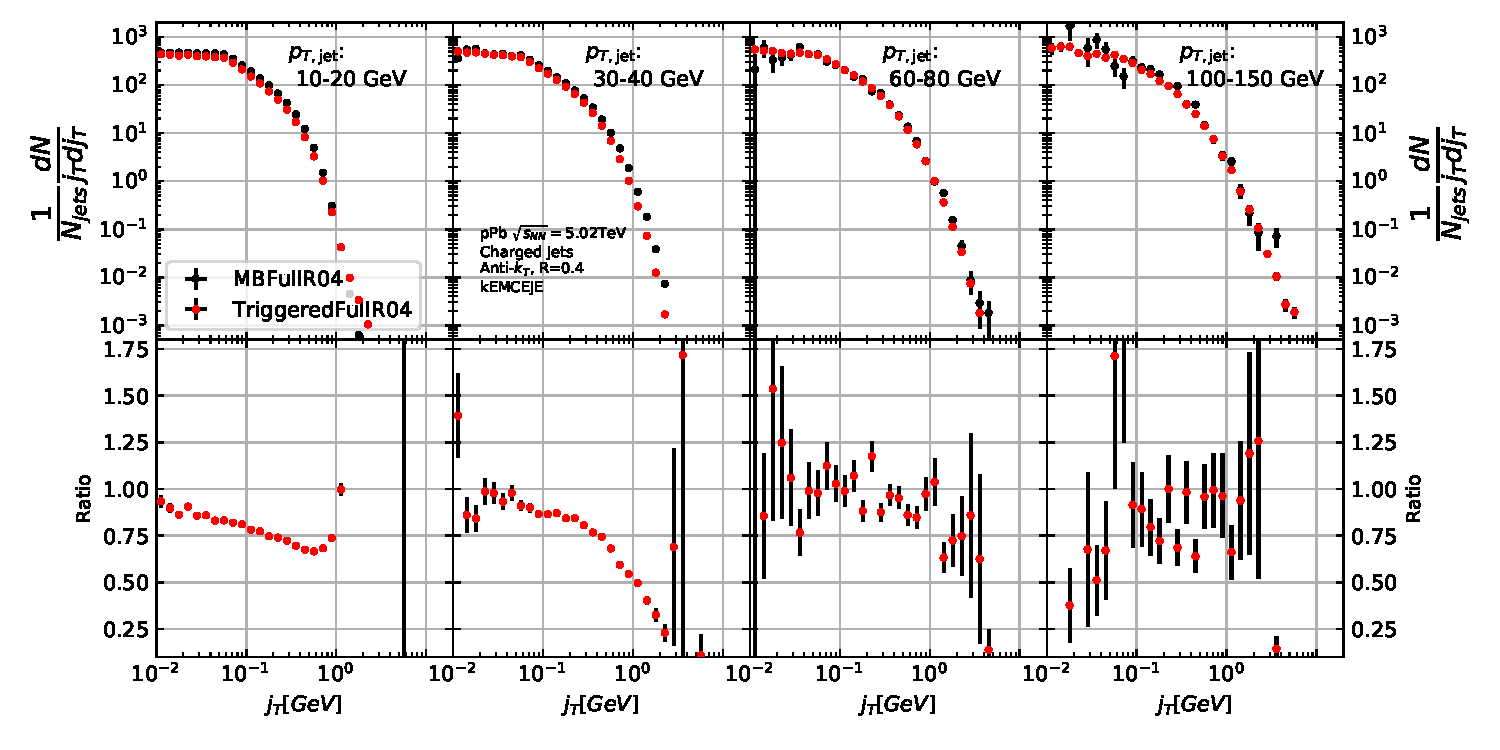
\includegraphics[width=0.95\textwidth]{results/MBvsTriggeredFullJetsR04JetConeJt.pdf} 
%%Tag 20170810 python2.7 Python/MBtoTriggeredComparison.py legotrain_CF_pPb-1053_20170223-2002_LHC13bcde.root
%
%%\includegraphics[width=0.95\textwidth]{results/OverlayjetjtIncl_T02_\figComment}
%\caption{Comparison between minimum bias and triggered datasets }
%%\end{subfigure}
%%\begin{subfigure}{0.5\textwidth}
%%%\includegraphics[width=0.95\textwidth]{results/OverlayjetjtIncl_T06_\figComment}
%%%\caption{Jet $\pt{}$ 80-100 GeV}
%%\end{subfigure}
%\end{figure}
%\subsection{Inclusive results}


%As outlined in Section ~\ref{sec:analysis} the inclusive $\jt{}$ distributions and corresponding backgrounds are obtained for different jet $\pt{}$ bins starting from $10\:\gev < \pt{,jet} < 20\:\gev$. Later the lowest $\pt{}$ bins are omitted because of problems in unfolding and fitting. The results are shown in Figure~\ref{fig:inclusive}. The background distribution the figure is obtained by the perpendicular cone method.







%\subsection{$\jt{} signal distributions$}
In this section I present the final results for $\jt{}$ signals. After unfolding and subtracting the background contribution we get the final $\jt{}$ distributions. Figure~\ref{fig:fits} shows $\jt{}$ distributions for two different $\pt{,jet}$ bins with $\unit[60]{\gev}< \pt{,jet}  < \unit[80]{\gev}$ and $\unit[100]{\gev}< \pt{,jet}  < \unit[150]{\gev}$. %Additional $\pt{,jet}$ bins are shown in appendix \ref{app:a}.
The distributions get wider with increasing $\pt{,jet}$. In part this is explained by kinematics; In a jet cone the cone size sets limits on the possible $\jt{}$ values. For a given $\pt{,track}$ the maximum $\jt{}$ value is approximately

\begin{equation}
\jt{max} \approx R\cdot \pt{,track},
\end{equation}

\noindent using the small angle approximation.


We fit the distribution using the two component fit function presented in Section~\ref{sec:fitting}. These are also shown in Figure~\ref{fig:fits}. Fitting a Gaussian alone to the entire $\jt{}$ distribution will produce a similar result as the Gaussian component in the two component fit. Thus the gaussian fit alone can't describe the full jet $\jt{}$ distribution. 


\begin{figure}[htb]
\centering
\begin{subfigure}{0.44\textwidth}
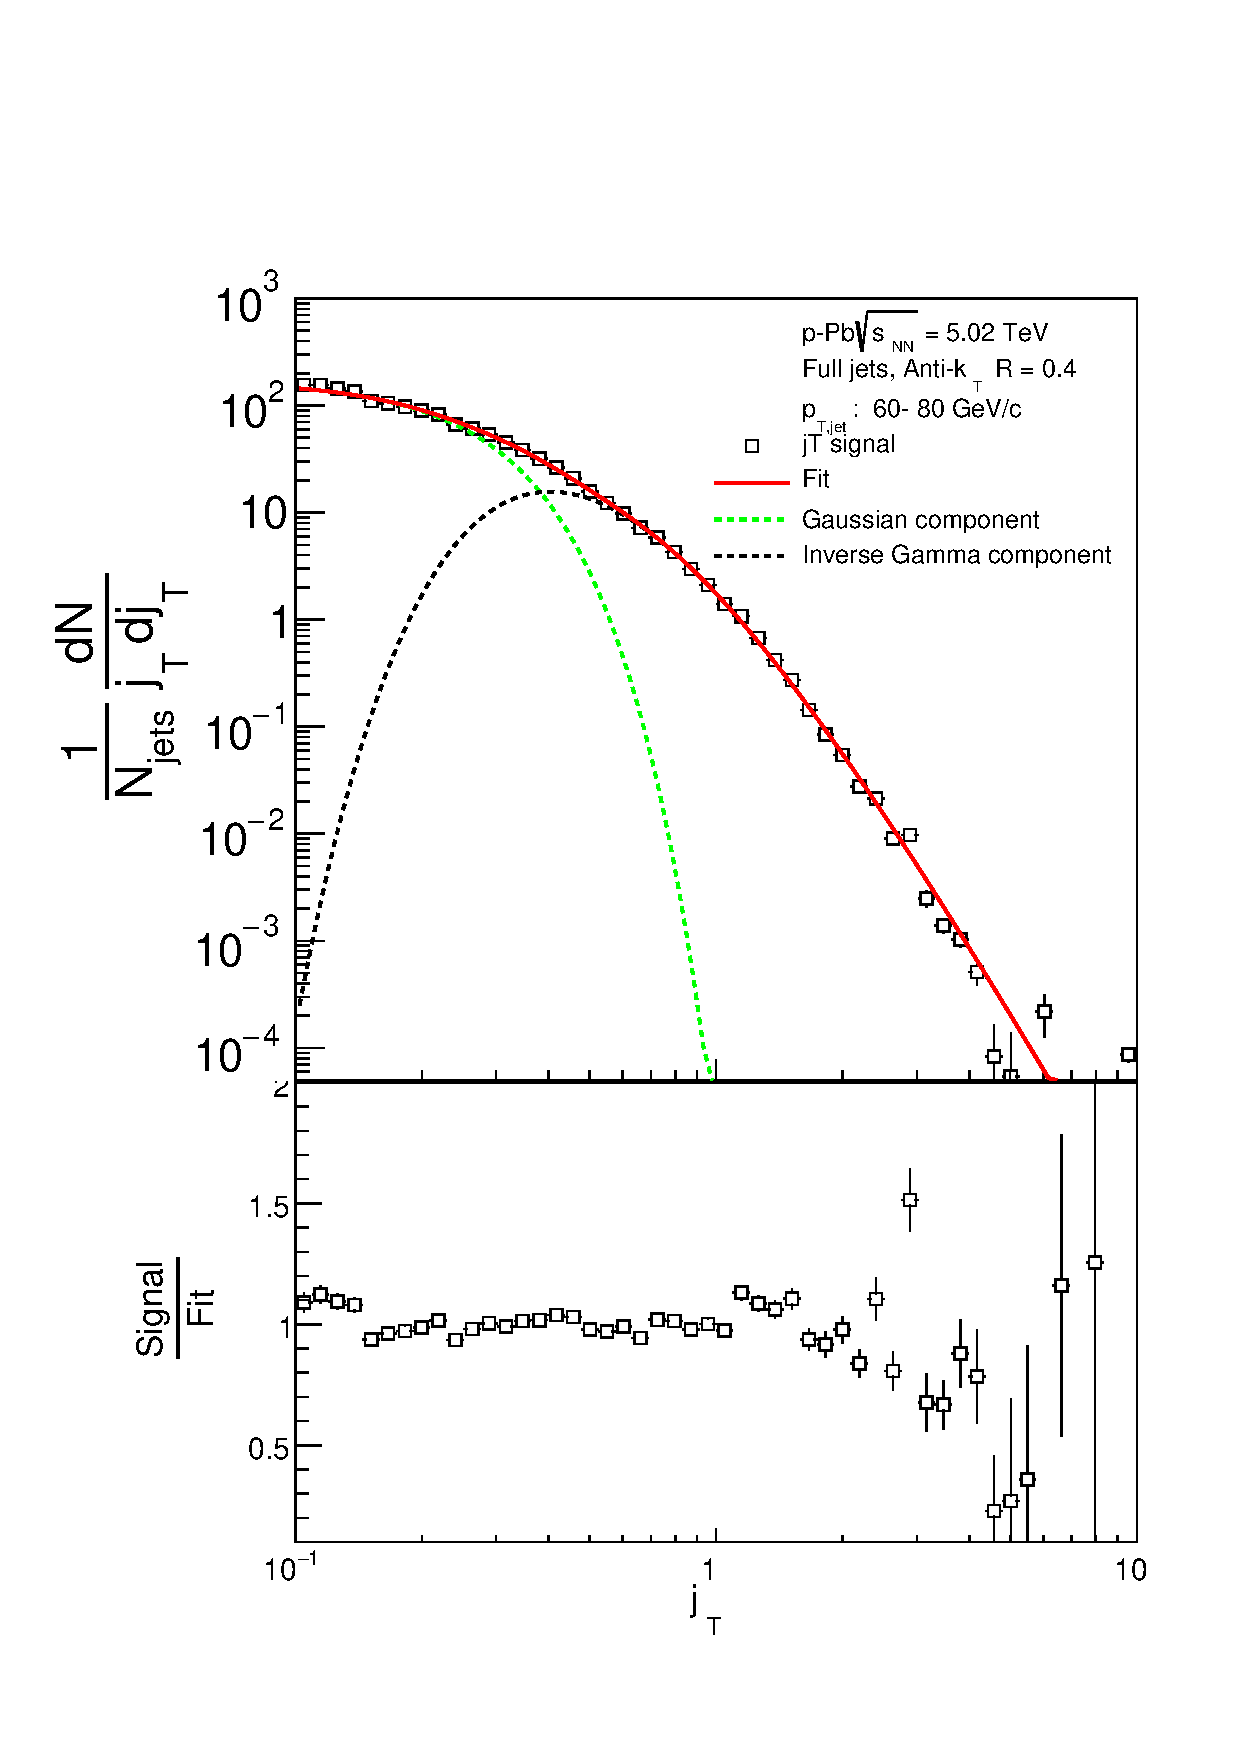
\includegraphics[width=0.95\textwidth]{results/JetConejTSignalFit/JetConejTSignalFitNFin00JetPt05perconeBgBayes}
\end{subfigure}
\begin{subfigure}{0.44\textwidth}
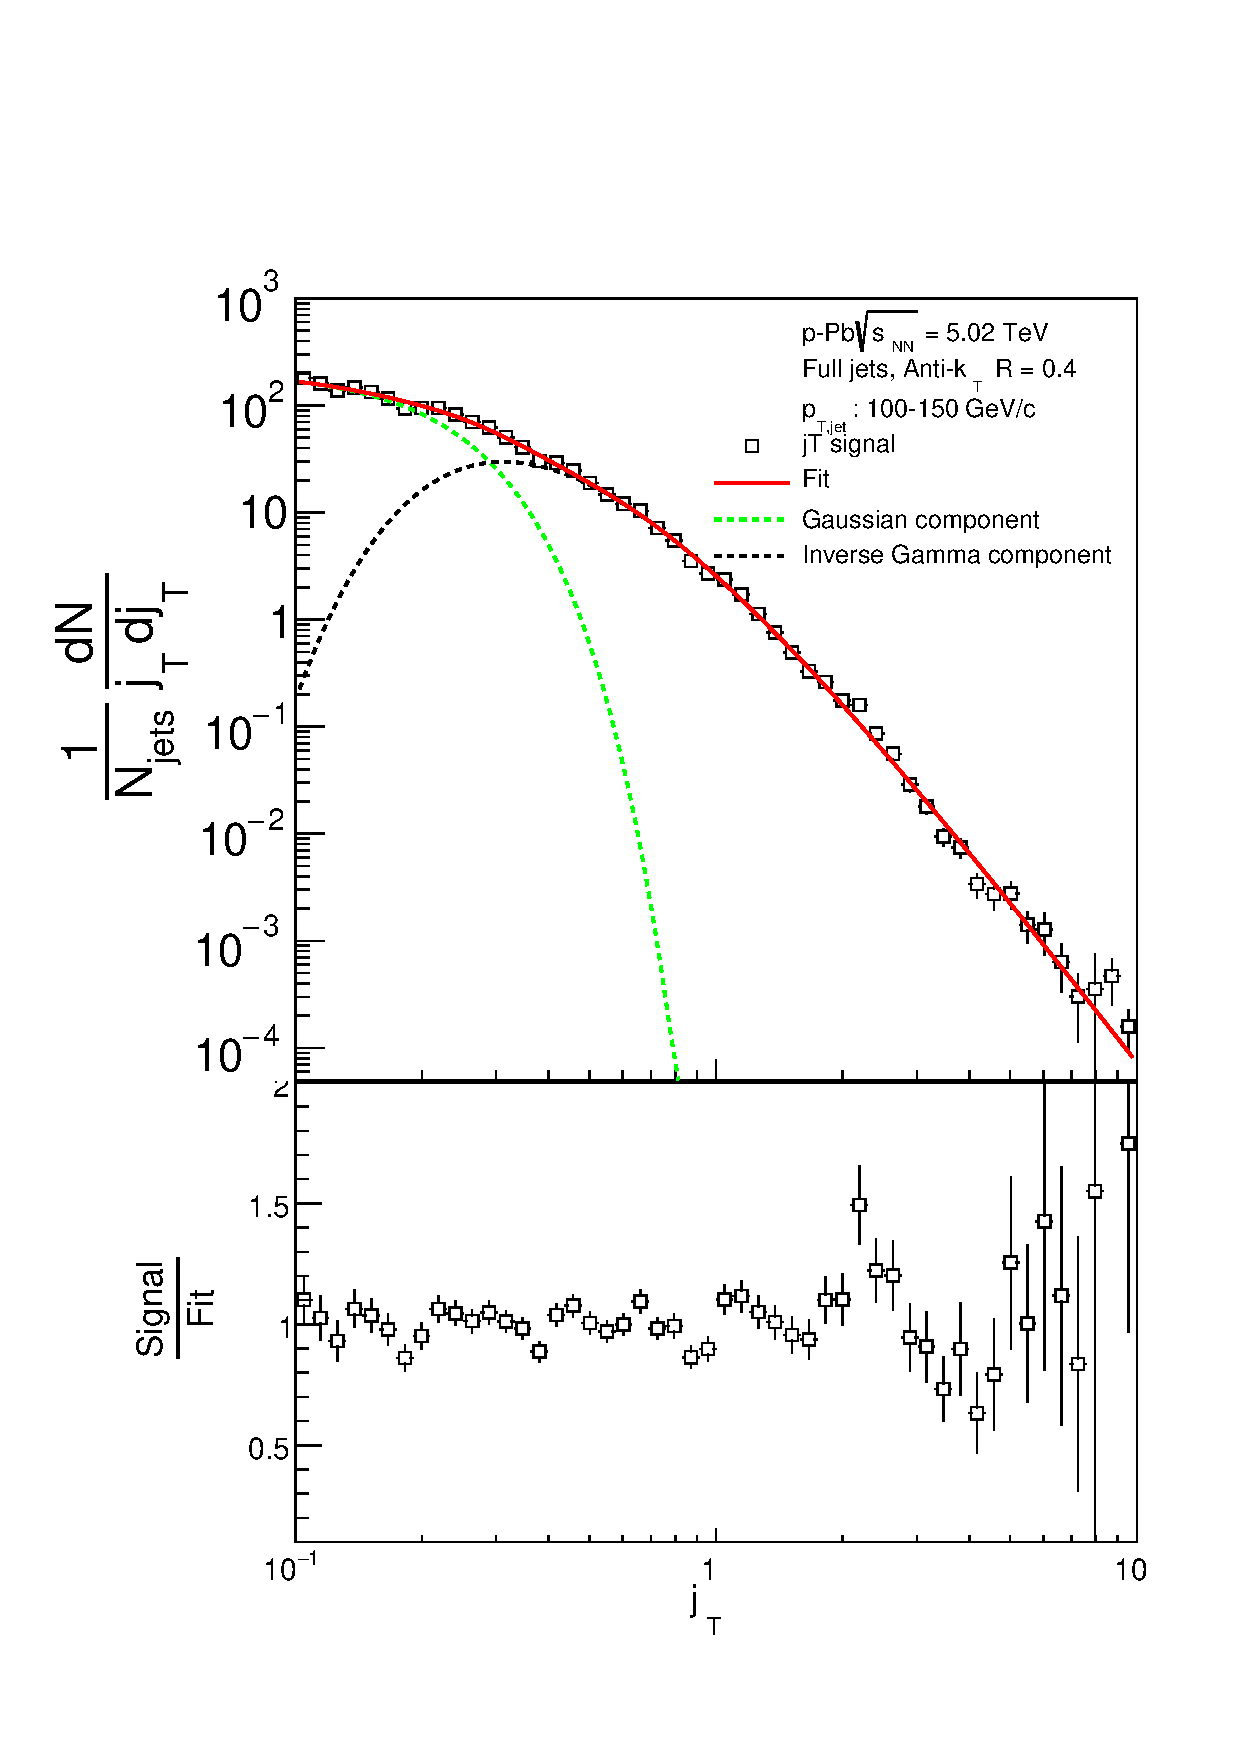
\includegraphics[width=0.95\textwidth]{results/JetConejTSignalFit/JetConejTSignalFitNFin00JetPt07perconeBgBayes}
\end{subfigure}
\caption{$\jt{}$ signal distributions fitted with the two component model are shown in different jet $\pt{}$ bins.}
\label{fig:fits}
\end{figure}

To characterise the widening of the $\jt{}$ distribution we can then extract the RMS, i.e. $\rms{\jt{}}$, values of the fits. Resulting RMS values with systematic errors are shown separately for the two components in Figure~\ref{fig:rms}. Here it is seen that the width of the narrow component shows only a weak dependence on the transverse momentum of the jet, $\pt{,jet}$. The RMS value of the wide component on the other hand increases with increasing $\pt{,jet}$.

The RMS values for both components are compared to \pythia~and Herwig simulations as shown in Figure~\ref{fig:pythia}. All the \pythia~models reproduce the data well, both the wide and narrow component.  For the narrow component Herwig gives RMS values comparable to the data. On the other hand, Herwig produces larger wide component $\rms{\jt{}}$ values than data and \pythia, and this difference seems to get larger with increasing $\pt{,jet}$.

\begin{figure}[htb]
\centering
%\begin{subfigure}{0.49\textwidth}
%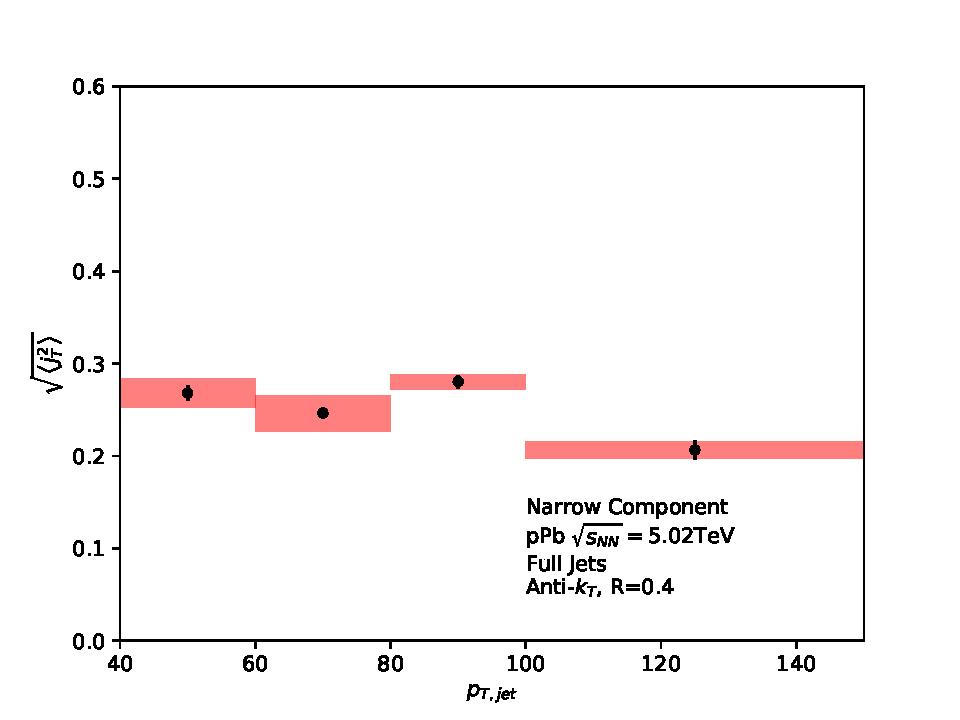
\includegraphics[width=0.95\textwidth]{results/gausRMSWithSystematics}
%\end{subfigure}
%%\begin{subfigure}{0.5\textwidth}
%%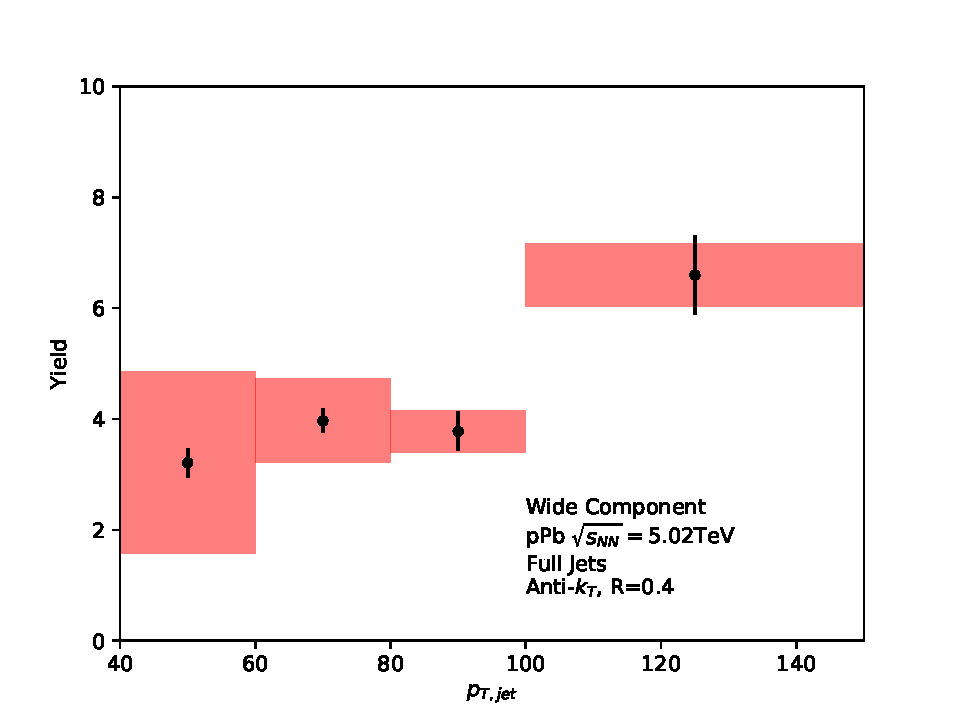
\includegraphics[width=0.95\textwidth]{results/gammaYieldWithSystematics}
%%\end{subfigure}
%\begin{subfigure}{0.49\textwidth}
%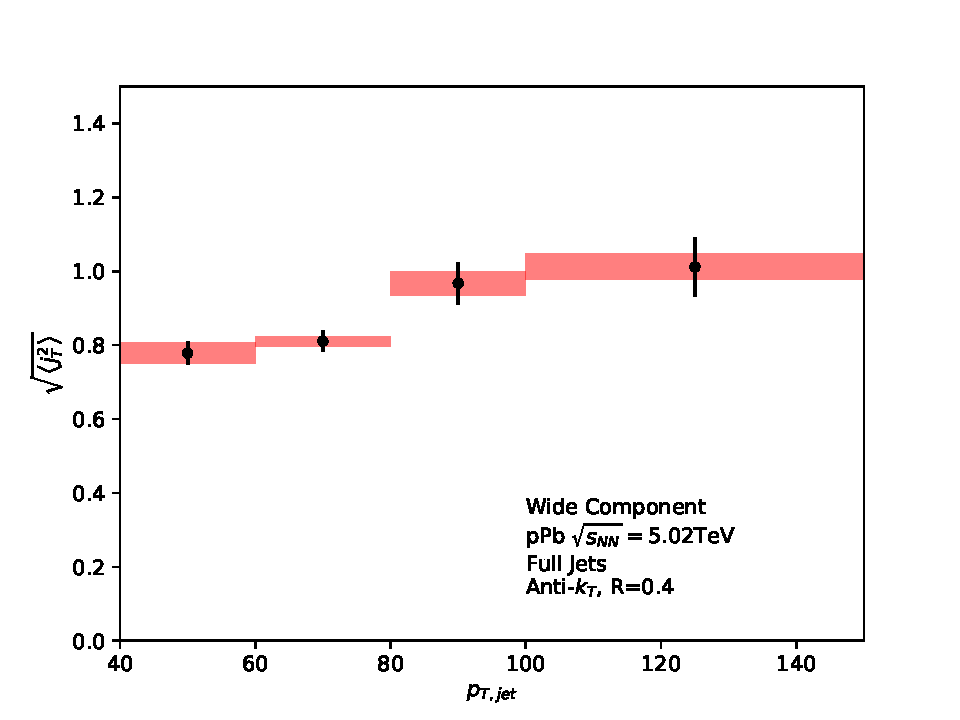
\includegraphics[width=0.95\textwidth]{figures/results/gammaRMSWithSystematics}
%\end{subfigure}
%%\begin{subfigure}{0.5\textwidth}
%%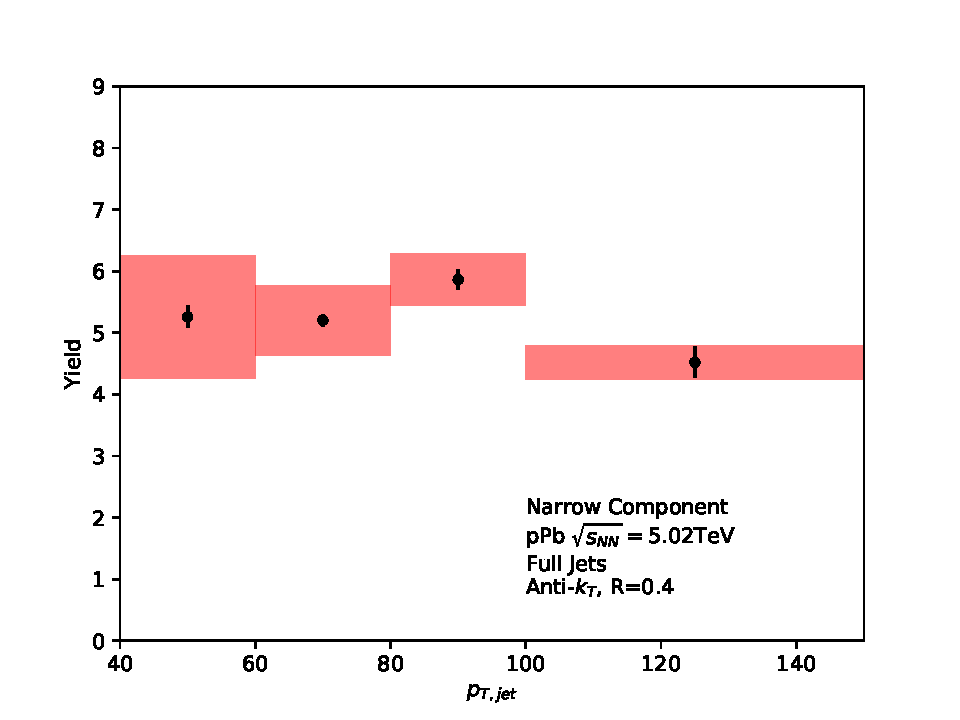
\includegraphics[width=0.95\textwidth]{results/gausYieldWithSystematics}
%%\end{subfigure}
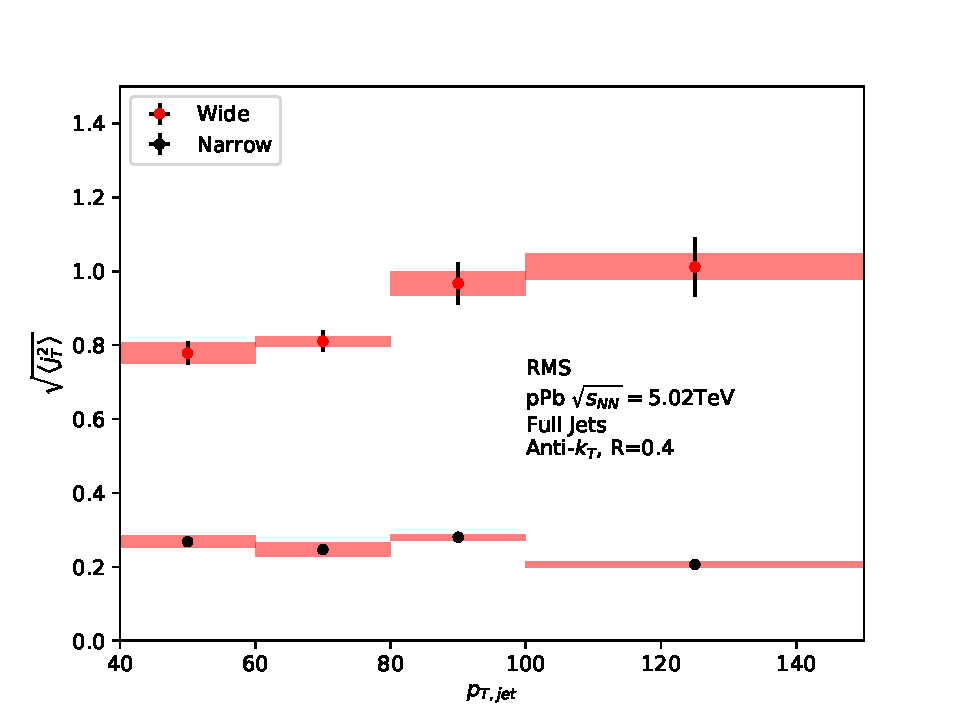
\includegraphics[width=0.65\textwidth]{figures/results/RMSWithSystematics}
\caption{RMS values extracted from the fits are shown for the Gaussian (narrow) and inverse gamma (wide) components.}
\label{fig:rms}
\end{figure}

\begin{figure}[htb]
\centering
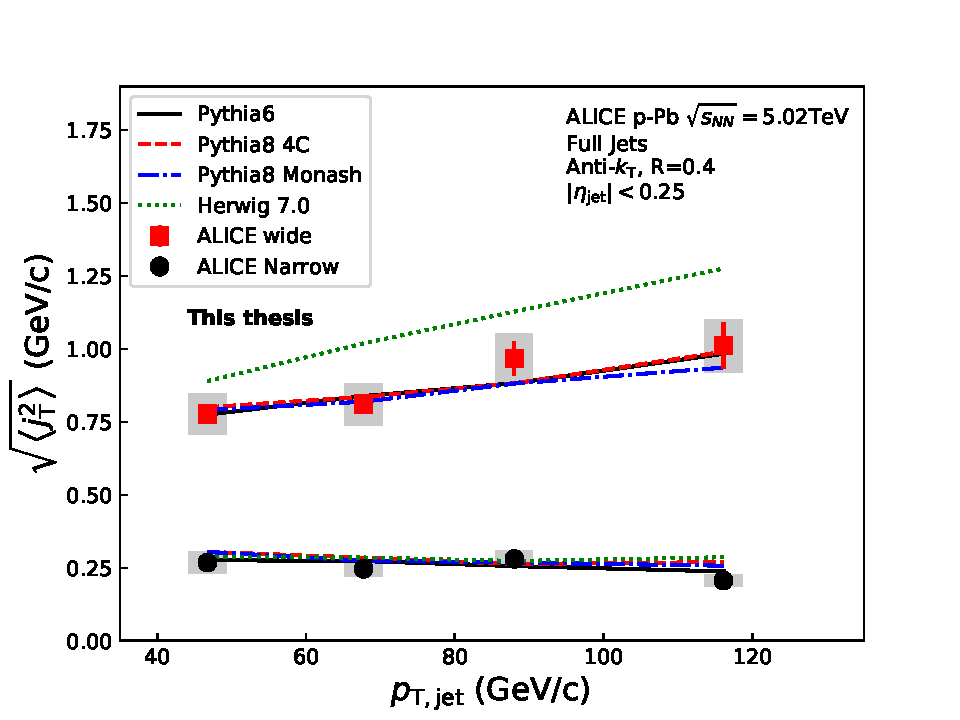
\includegraphics[width=0.65\textwidth]{figures/results/RMSWithSystematics_Pythia}
\caption{RMS values extracted from the fits are compared to Monte Carlo models. \pythia~ reproduces the data well for both the narrow and wide components. Herwig produces wider distributions. }
\label{fig:pythia}
\end{figure}
\FloatBarrier
\subsection{High multiplicity events}

\begin{figure}[htb]
\centering
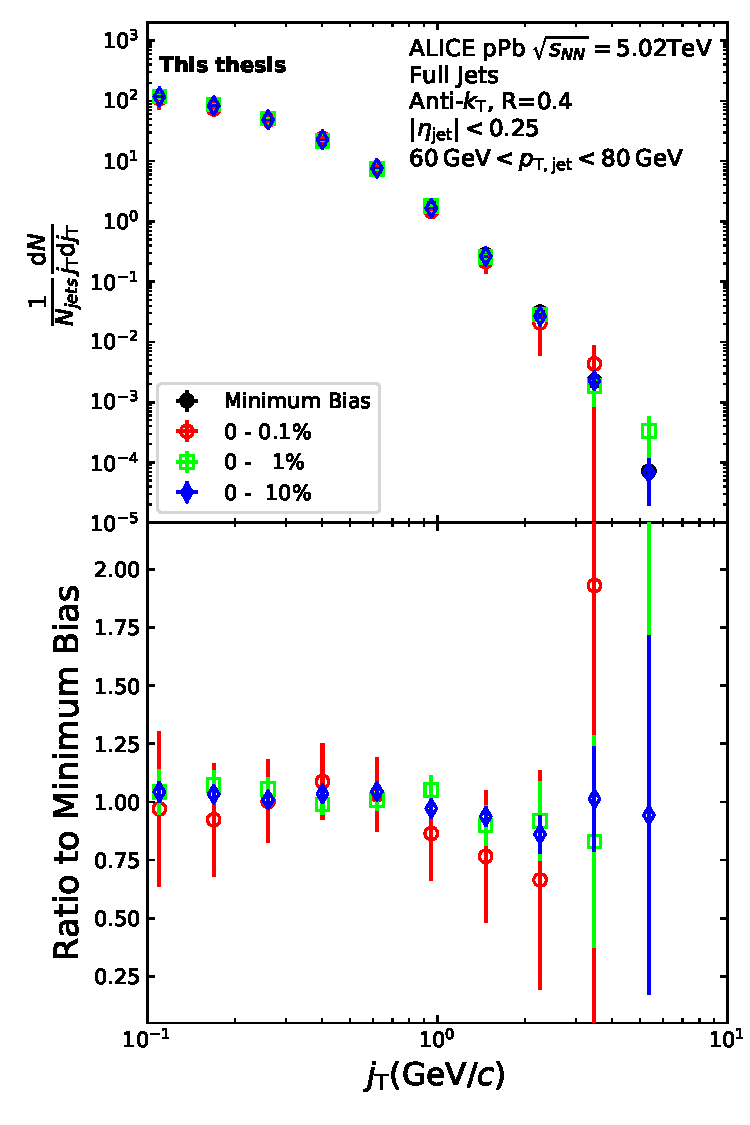
\includegraphics[width=0.75\textwidth]{figures/results/HighMJetConeJtSignalPtFrom4To5.pdf}
\caption{$\jt{}$ distributions are shown for various multiplicity bins in \pPb collisions.}
\label{fig:highm}
\end{figure}

The analysis was repeated taking only events with high multiplicity. Three different multiplicity percentile cuts were used; \unit[10]{\%}, \unit[1]{\%} and \unit[0.1]{\%}. The centrality estimations were given by the V0A estimator. Resulting $\jt{}$ signal distributions are shown in Figure~\ref{fig:highm}. From the figure one can observe no modification within the errors when tighter multiplicity cuts are introduced. %We used ZDC({\color{red}TODO}) as a centrality estimator. As argued in Section~\ref{sec:smallsystemcentrality} the zero-degree energy deposit should provide a centrality estimator with minimal bias from jet production, as it should be measure of the number of spectator nucleons. 
 %There is a small dip at $\jt{} \approx 2$, but it is within the statistical errors. This is also the region where the signal is most sensitive to background subtraction. Higher multiplicity events will naturally have a higher background contribution. Background estimation is done separately for the multiplicity bins. Thus it is not expected that different backgrounds would cause a difference, but this possibility can't be ruled out.

As described in Section~\ref{sec:smallsystem} no conclusive evidence of jet modification in \pPb collisions has been observed. However, all previous observations have been done for minimum bias events. Most observables are based on measuring yield instead of jet shape and are thus sensitive to biases in the centrality selection. No previous jet shape measurements have been performed in high multiplicity \pPb events, where collective motion was observed.

%Thus any difference in $\jt{}$ would also be small. 

As the statistics are limited in the high multiplicity runs, it was hard to achieve stable fits to the distributions. Thus the RMS values are not shown. 



